%\begin{table}[h!]
%\begin{center}

\section{Spannungsreferenzen}
% % % % % % % % % % % % % % % % % % %
% %Spannungsteiler
% % % % % % % % % % % % % % % % % % %
\subsection{Spannungsteiler}

 	\begin{minipage}{150pt}
	 	{ \begin{circuitikz}[scale = 0.6, transform shape]

\draw 
%Titel des Bildes
node (text) at (0, -1)  {\textbf{spannungsteiler}}
% alle Knoten
node  (VDD) at (0, 4)  {}
node  (a)   at (0, 2)  {}
node  (ref) at (1, 2)  {}
node  (gnd1)at (0, 0)  {}
node  (gnd2)at (1, 0)  {}

% Knoten anschreiben
(VDD) node[left] {$V_{DD}$}

%Verbindungen
(VDD)  to [european resistor,o-, l = $R_1$] (a)
       to [european resistor,*-, l = $R_2$] (gnd1)
(a)    to [short](ref)
(gnd2) to [open, -o, v = $U_{ref}$] (ref)
(gnd2) to [short, o-*] (gnd1)
%Knoten zeichen, gnd und so     
node[ground] at (gnd1) {};



\end{circuitikz}
 }
 	\end{minipage}
 	\begin{minipage}{150pt}
	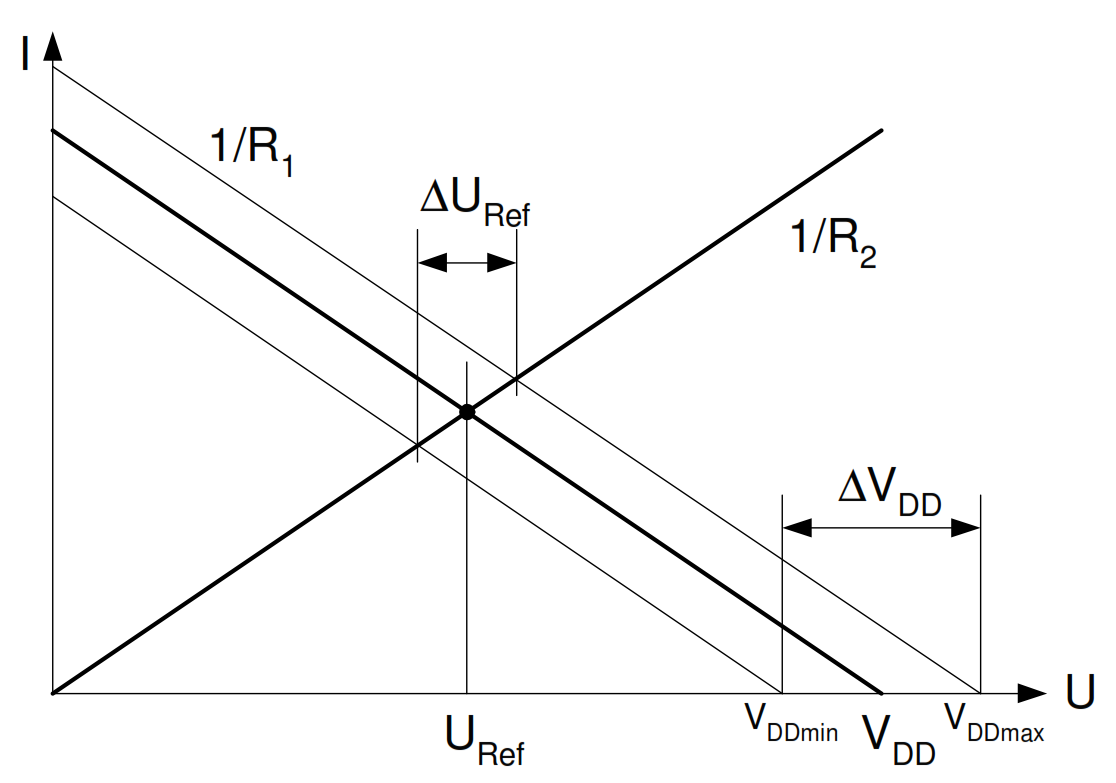
\includegraphics[width = 4cm]{images/spgref/05_spgteiler}
 	\end{minipage}
 	\begin{minipage}{200pt}
		\emph{Sensitivität}, empfindlichkeit gegenüber Speisespannungsschwankung:\newline $\underset{V_{DD}}{\overset{U_{Ref}}{S}} = \dfrac{\Delta  U_{Ref}/ U_{Ref}}{\Delta V_{DD}/V{DD}} = 1$\newline
		$U_{Ref} = V_{DD}\dfrac{R2}{R1+R2}$
	\end{minipage}\\
% % % % % % % % % % % % % % % % % % %
% %Spannungsteiler pnp
% % % % % % % % % % % % % % % % % % %
\subsection{Diodenreferenz}
	\begin{minipage}{100pt}
	\begin{circuitikz}[scale=0.5, transform shape]

\draw 
%Titel des Bildes
node (text) at (0, -1)  {\textbf{spagteiler mit pn Übergang}}
% alle Knoten
node  (VDD) at (0, 4)  {}
node  (a)   at (0, 2)  {}
node  (ref) at (1, 2)  {}
node  (gnd1)at (0, 0)  {}
node  (gnd2)at (1, 0)  {}

% Knoten anschreiben
(VDD) node[left] {$V_{DD}$}

%Verbindungen
(VDD)  to [european resistor,o-, l = $R_1$] (a)
       to [Do,*-, l = $D_2$] (gnd1)
(a)    to [short](ref)
(gnd2) to [open, -o, v = $U_{ref}$] (ref)
(gnd2) to [short, o-*] (gnd1)
%Knoten zeichen, gnd und so     
node[ground] at (gnd1) {};


\end{circuitikz}

	\end{minipage}
	\begin{minipage}{150pt}
	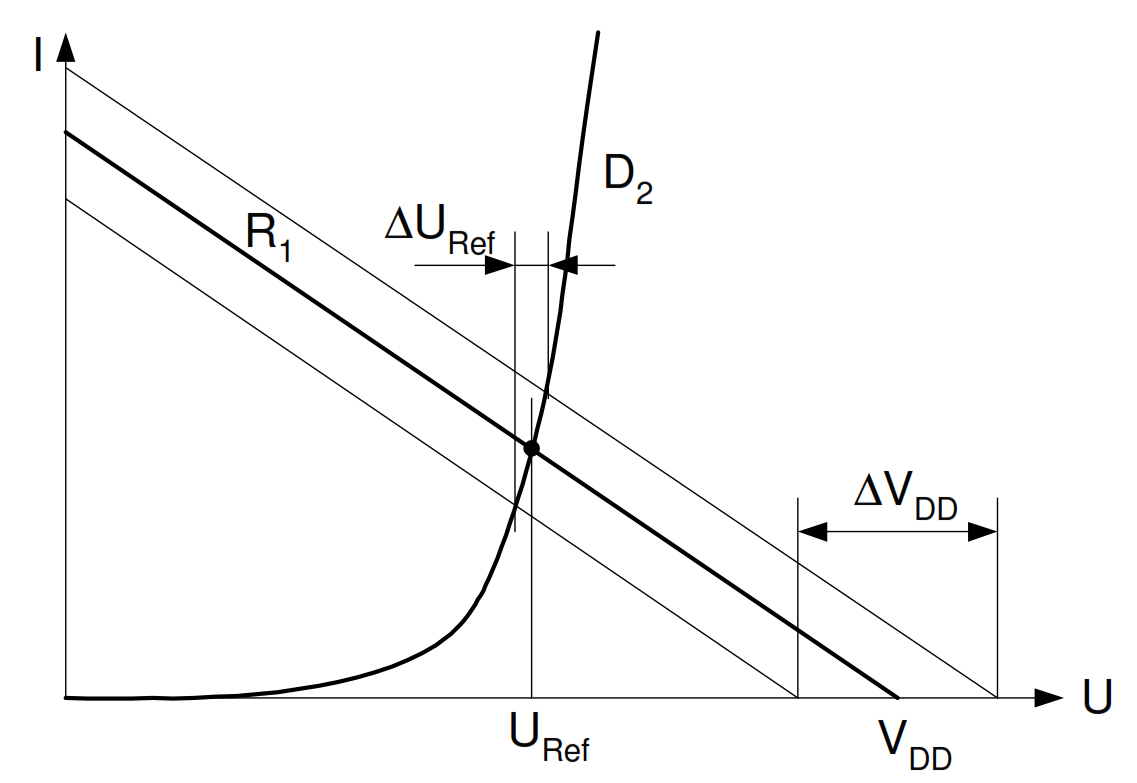
\includegraphics[width = 4cm]{images/spgref/06_diodenref}
	\end{minipage}
	\begin{minipage}{200pt}
	$U_{Ref} =  \dfrac{kT}{q}\ln\left(\dfrac{I}{I_s}\right) = V_T\cdot \ln\left(\dfrac{I}{I_s}\right)$\newline
	$\underset{V_{DD}}{\overset{U_{Ref}}{S}} = \dfrac{1}{\ln\left(\dfrac{I}{I_S}\right)}<1$\newline
	Diff. Widerstand: $r_D=\dfrac{m\cdot V_T}{I}$
	$k = 1.38\cdot 10^{-23} \frac{J}{K},\newline
	 T = \text{absolute Temperatur} [K], \newline
	 q = 1.602\cdot 10^-{19}As, \newline
	 I_s = \text{Sperrstrom}, \newline
	 V_T = 25.5mV$	\\
	\end{minipage}
\hrule
% % % % % % % % % % % % % % % % % % %
% %Bootstrap
% % % % % % % % % % % % % % % % % % %
\subsection{PTAT(Proportional to absolute temperature) , Bootstrap Referenz}
	\begin{minipage}{200pt}
		\begin{circuitikz}[scale = 1, transform shape]
\draw 

%Titel des Bildes
node (text) at (1, 0.2)  {\textbf{Bootstrap}}
% alle Bauteile
(0,6) node [ pmos, rotate=180, transform shape] (M3) {}
(M3) node[left] {$M_3$}

(2.5,6) node [ pmos] (M4) {}
(M4) node[right] {$M_4$}

(4,5) node [ pmos] (M5) {}
(M5) node[right] {$M_5$}

(0,4) node [ nmos, rotate=180, transform shape] (M1) {}
(M1) node[left] {$M_1$}

(2.5,4) node [ nmos] (M2) {}
(M2) node[right] {$M_2$}

(0,2) node [ pnp, , rotate=180, transform shape] (Q1) {}
(Q1) node[left] {$Q_1$}

%Spannungslinien
(0,7) to [short, l=$V_{DD}$] (4,7)
(0,1) to [short, l_=GND] (4,1)

%verbindungen 
(M3.D) to [short] (0,7)
(M4.S) to [short, -*] (2.5,7)
(M3.S) to [short,i =$i_1$ ](M1.S)

(M1.S) to [short, *-] (1.35,4.75)
(1.35,4.75) to[short ,-*] (1.35, 4)

(M1.G) to [short] (M2.G)
(M1.D) to (Q1.C)

(Q1.E) to (0,1)
(Q1.B) to [short, -*] (0.85,1)

(M4.D) to (M2.D)
(M2.S) to [european resistor, l=$R$, -*] (2.5,1)
(M5.S) to [short, -*](4,7)
(M5.G) to [short, -*] (2.5,5)
(M5.D) to [short, i=$i_5$] (4,3) 
(M3.G) to (M4.G)
(2.5,4.6) to [short, i = $i_2$] (2.5, 4.5)
;





\end{circuitikz}



	\end{minipage}
	\begin{minipage}{300pt}
	Die Bootstrap Referenz ist unabhängig von $V_{DD}$, dafür temperaturabhängig, 2 mögliche Arbeitspunkte, Startup-Schaltung benötigt\newline
	$I_1 = I_2 = I_5 \qquad V_{EB1} = V_R  $\newline
	$V_{EB1} = m\cdot V_T \ln \left(\dfrac{I_1}{I_S}\right) = I_2 R$\newline
	Temp. koeffizient: $T_C = \dfrac{1}{V_T}\cdot \dfrac{dV_T}{dT} = \dfrac{1}{T}$
	\end{minipage}\\
\hrule
% % % % % % % % % % % % % % % % % % % %
% %Technologie unabhängige VT-Referenz
% % % % % % % % % % % % % % % % % % % %
\subsection{Technologie unabhängige $V_T$-Referenz}
	\begin{minipage}{150pt}
	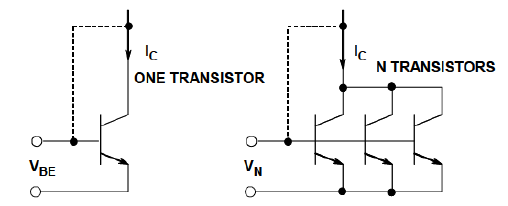
\includegraphics[width = 6cm]{images/spgref/01_vtref.png}
		%  not finished tikz tikz/04_techunabh}}&
	\end{minipage}
	\begin{minipage}{150pt}
	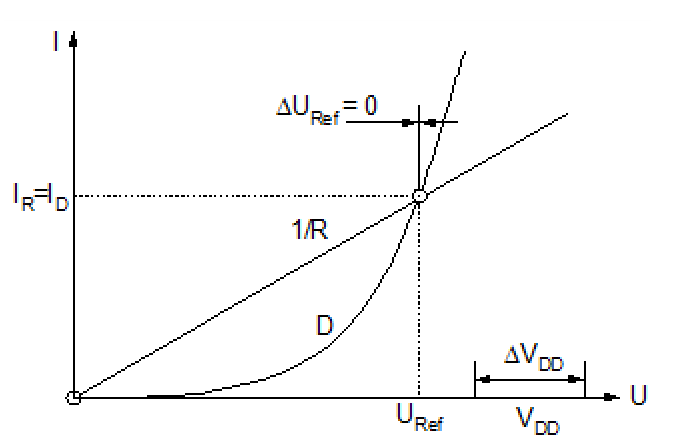
\includegraphics[width = 4cm]{images/spgref/02_vtref_diag.png}
	\end{minipage}
	\begin{minipage}{200pt}
	Technologie unabhängige $V_T$ Referenzen hängen nur von der Geometrie der Transistoren ab(Anzahl paralleller Trans.). Sie Werden zur Messung der Temperatur eingesetzt.\newline
	$V_N = \dfrac{kT}{q}\ln\left(\dfrac{I_C}{N\cdot I_S}\right) $ \newline
	$V_{BE} =\dfrac{kT}{q}\ln\left(\dfrac{I_C}{I_S}\right)$\newline
	$\Delta V_{BE} = V_{BE} -V_N = \dfrac{kT}{q}\ln(N)$
	\end{minipage}
% % % % % % % % % % % % % % % % % % %
% %Bandgap-Referenzen
% % % % % % % % % % % % % % % % % % %
\subsection{Bandgap Referenzen}
	\begin{minipage}{250pt}
		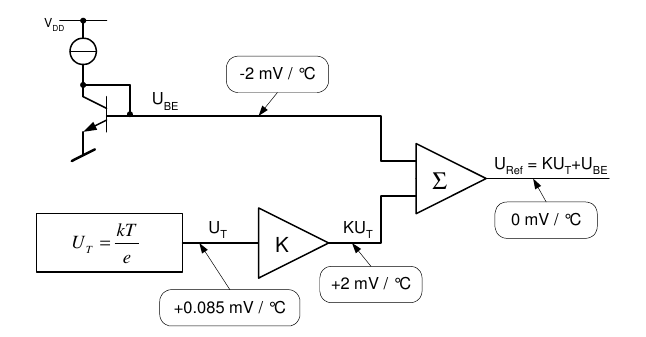
\includegraphics[width = 8cm]{./images/spgref/03_bandgap.png}
	\end{minipage}
 	\begin{minipage}{250pt}
 	Bandgap-Referenzen können Temperaturkoeffizienten von 10-100 ppm/°C über einen Temperaturbe-
 	reich von 0 °C bis 70 °C erreichen.
 	\end{minipage}
% % % % % % % % % % % % % % % % % % %
% %Variable Referenzen
% % % % % % % % % % % % % % % % % % %
\subsection{Variable Referenzen}
	\begin{minipage}{150pt}
		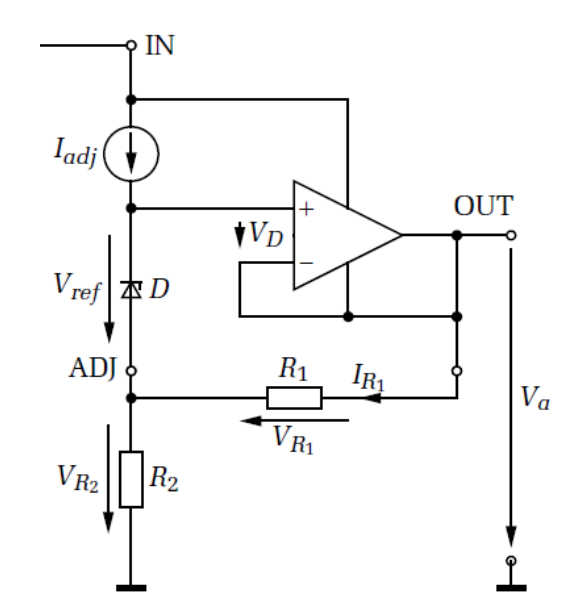
\includegraphics[width = 5cm]{./images/spgref/04_var_ref.png}
	\end{minipage}
	\begin{minipage}{300pt}
	Adjust-Pin (ADJ) zum Anschluss der externen Widerstände $R_1, R_2$\\
		$V_{R1} = V_{REF} \qquad I_{R1} = I_{ADJ} \qquad V_{OUT} = V_{REF}\left(1+\dfrac{R_2}{R_1}\right)+I_{adj}\cdot R_2$\newline
	für $I_{adj} << I_{R1}$ gilt\\
	$V_{OUT} = V_{REF}\cdot \left(1+\dfrac{R_2}{R_1}\right)$
	\end{minipage}	 
	
